%! alt Trapezium ABCD with AB parallel to CD. The circles on the legs AD and BC as diameters, centred at their midpoints M and N, touch at P on the midline MN. Segments PA = 75, PD = 100, PB = 65 and PC = 156 make right angles APD and BPC. A dashed circle of radius 60 centred at P touches all four sides: P is the centre of the inscribed circle.
%! after_paragraph 2
%! scale 1/40
% The shared preamble of every Cevian figure. pipeline/figures turns these colours into theme-aware paint,
% and refuses any other colour, so draw only with them:
%   figink (lines and labels), figaux (construction lines), figaccent (the object the argument turns on),
%   figtint and figaccenttint (light fills).
\documentclass[border=1.5pt]{standalone}
\usepackage{tkz-euclide}
\definecolor{figink}{RGB}{0,0,0}
\definecolor{figaux}{RGB}{85,85,85}
\definecolor{figaccent}{RGB}{192,57,43}
\definecolor{figtint}{RGB}{221,221,221}
\definecolor{figaccenttint}{RGB}{245,213,208}
% tkz-euclide's defaults draw circles, compasses and marks in 50% grey and fill points with a tint.
\makeatletter
\def\tkz@otherlinecolor{figink}
\def\tkz@euc@circlecolor{figink}
\def\tkz@euc@compasscolor{figink}
\def\tkz@euc@mkcolor{figink}
\def\tkz@mk@fill{figink}
\def\tkz@euc@pointfillcolor{figink}
\makeatother
\tkzSetUpLine[color=figink,line width=.7pt]
\tkzSetUpArc[color=figink,line width=.7pt]
\tkzSetUpCompass[color=figink,line width=.5pt]
\tkzSetUpPoint[color=figink,fill=figink,size=3.1pt]
\tikzset{
  every picture/.style={line cap=round,line join=round,color=figink},
  circle style/.append style={color=figink,line width=.7pt},
  aux/.style={color=figaux,line width=.45pt,dash pattern=on 2.6pt off 2pt},
  key/.style={color=figaccent,line width=1pt},
  mk/.style={color=figink,line width=.5pt},
  lbl/.style={color=figink,inner sep=2.2pt},
  len/.style={color=figink,inner sep=1.5pt,font=\small},
}

\begin{document}
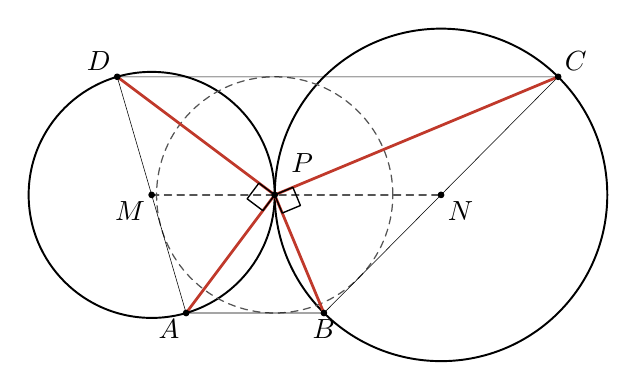
\begin{tikzpicture}
\tkzDefPoint(-1.1250000,0.0){A} %! A = (-45, 0)
\tkzDefPoint(0.62500000,0.0){B} %! B = (25, 0)
\tkzDefPoint(3.6000000,3.0000000){C} %! C = (144, 120)
\tkzDefPoint(-2.0000000,3.0000000){D} %! D = (-80, 120)
\tkzDefPoint(0.0,1.5000000){P} %! P = (0, 60)
\tkzDefPoint(-1.5625000,1.5000000){M} %! M = (-125/2, 60)
\tkzDefPoint(2.1125000,1.5000000){N} %! N = (169/2, 60)
\tkzDefPoint(0.0,0.0){T} %! T = (0, 0)
\tkzDefPoint(0.35000000,1.9000000){Lp} %! Lp = (14, 76)
%! fact parallel(A, B, D, C)
%! fact midpoint(M, A, D)
%! fact midpoint(N, B, C)
%! fact tangent_circles(M, dist(A, D)/2, N, dist(B, C)/2)
%! fact on_circle(P, M, dist(A, D)/2)
%! fact on_circle(P, N, dist(B, C)/2)
%! fact on_segment(P, M, N)
%! fact dist(P, A) == 75
%! fact dist(P, D) == 100
%! fact dist(P, B) == 65
%! fact dist(P, C) == 156
%! fact perp(P, A, P, D)
%! fact perp(P, B, P, C)
%! fact dist(P, foot(P, A, B)) == 60
%! fact dist(P, foot(P, D, C)) == 60
%! fact dist(P, foot(P, A, D)) == 60
%! fact dist(P, foot(P, B, C)) == 60
%! fact equal(dist(A, B) + dist(C, D), dist(A, D) + dist(B, C))
%! fact on_circle(T, P, 60)
\tkzDrawCircle(M,A)
\tkzDrawCircle(N,B)
\tkzDrawCircle[aux](P,T)
\tkzDrawSegment[aux](M,N)
\tkzDrawPolygon(A,B,C,D)
\tkzDrawSegments[key](P,A P,D P,B P,C)
\tkzMarkRightAngle[size=.25,mk](A,P,D)
\tkzMarkRightAngle[size=.25,mk](B,P,C)
\tkzDrawPoints(A,B,C,D,P,M,N)
\tkzLabelPoint[below left,lbl](A){$A$}
\tkzLabelPoint[below,lbl](B){$B$}
\tkzLabelPoint[above right,lbl](C){$C$}
\tkzLabelPoint[above left,lbl](D){$D$}
\tkzLabelPoint[lbl,anchor=center](Lp){$P$}
\tkzLabelPoint[below left,lbl](M){$M$}
\tkzLabelPoint[below right,lbl](N){$N$}
\end{tikzpicture}
\end{document}
